%!TEX root = ../thesis_a4.tex
% Some new commands for setting up appendices
\newcommand\contrib[1]{\\~{\footnotesize (#1)}}
% 
\newcommand\resource[2]{
	\noindent #1 \par
	\vspace{0.2em}
	{\centering	\url{#2} \par}
	\vspace{0.5em}
	\hrule \par 
	\vspace{0.8em} \par}
%
%
\chapter[Publications by the author][Publications by the author]{Publications by the author}\label{app:mypapers}% by the author

We here provide a list of publications by the author related with the thesis work. For the publications where the role is not that of the first author we  also specify the contributions. Wherever not specified, the contributions are mainly in the formulation of the research problem, building the dataset, writing the code, performing the experiments, analyzing the results and writing the manuscript.

\subsection*{Peer-reviewed journals}
\begin{itemize}[leftmargin=*]
	\item \textbf{Gulati, S.}, Bellur, A., Salamon, J., Ranjani, H., Ishwar, V., Murthy, H. A., \& Serra, X. (2014). Automatic tonic identification in Indian art music: approaches and evaluation. \textit{Journal of New Music Research}, 43(1), 53–71.
	\contrib{Companion webpage: \url{http://compmusic.upf.edu/node/323}}
	\item Koduri, G. K., \textbf{Gulati, S.}, Rao, P., \& Serra, X. (2012). R\={a}ga recognition based on pitch distribution methods. \textit{Journal of New Music Research}, 41(4), 337–350.
	\contrib{Formulating methodology, Writing parts of the code}
	
\end{itemize}
%
\subsection*{Full articles in peer-reviewed conferences}
\begin{itemize}[leftmargin=*]
	\item \textbf{Gulati, S.}, Serr{\`a}, J., Ganguli, K. K., \c{S}ent{\"u}rk, S., \& Serra, X. (2016). Time-delayed melody surfaces for r\={a}ga recognition. In \textit{Proceedings of the 17th International Society for Music Information Retrieval Conference (ISMIR)}, pp. 751–757. New York, USA.
	\contrib{Companion webpage: \url{http://compmusic.upf.edu/node/300}}
	%
	\item Ganguli, K. K., \textbf{Gulati, S.}, Serra, X., \& Rao, P. (2016). Data-driven exploration of melodic structures in Hindustani music. In \textit{Proceedings of the 17th International Society for Music Information Retrieval Conference (ISMIR)}, pp. 605-611. New York, USA.
	\contrib{Formulation of the problem, building dataset, writing the code, writing the manuscript.}
	%
	\item \textbf{Gulati, S.}, Serr{\`a}, J., Ishwar, V., \c{S}ent{\"u}rk, S., \& Serra, X. (2016). Phrase-based r\={a}ga recognition using vector space modeling. In \textit{Proceedings of the 41st IEEE International Conference on Acoustics, Speech and Signal Processing (ICASSP)} , pp. 66–70. Shanghai, China.
	\contrib{Companion webpage: \url{http://compmusic.upf.edu/node/278}}
	%
	\item \textbf{Gulati, S.}, Serr{\`a}, J., Ishwar, V., \& Serra, X. (2016). Discovering r\={a}ga motifs by characterizing communities in networks of melodic patterns. In \textit{Proceedings of the 41st IEEE International Conference on Acoustics, Speech and Signal Processing (ICASSP)}, pp. 286–290. Shanghai, China.
	\contrib{Companion webpage: \url{http://compmusic.upf.edu/node/277}}
	%
	\item \textbf{Gulati, S.}, Serr{\`a}, J., \& Serra, X. (2015). Improving melodic similarity in Indian art music using culture-specific melodic characteristics. In \textit{Proceedings of the 16th International Society for Music Information Retrieval Conference (ISMIR)}, pp. 680–686. M{\'a}laga, Spain.
	\contrib{Companion webpage: \url{http://compmusic.upf.edu/node/269}}
	%
	\item \textbf{Gulati, S.}, Serr{\`a}, J., \& Serra, X. (2015). An evaluation of methodologies for melodic similarity in audio recordings of Indian art music. In \textit{Proceedings of the 40th IEEE International Conference on Acoustics, Speech and Signal Processing (ICASSP)}, pp. 678–682. Brisbane, Australia.
	\contrib{Companion webpage: \url{http://compmusic.upf.edu/node/242}}
	%
	\item \textbf{Gulati, S.},  Serr{\`a}, J., Ishwar, V., \& Serra, X. (2014). Mining melodic patterns in large audio collections of Indian art music. In \textit{Proceedings of the International Conference on Signal Image Technology \& Internet Based Systems (SITIS-MIRA)}, pp. 264–271. Marrakesh, Morocco.
	\contrib{Companion webpage: \url{http://compmusic.upf.edu/node/210}}
	%
	\item \textbf{Gulati, S.}, Serr{\`a}, J., Ganguli, K. K., \& Serra, X. (2014). Landmark detection in Hindustani music melodies. In \textit{Proceedings of the International Computer Music Conference / Sound and Music Computing Conference (ICMC-SMC)}. Athens, Greece. 
	\contrib{Companion webpage: \url{http://compmusic.upf.edu/node/324}}
	%
	\item Srinivasamurthy, A., Koduri, G. K., \textbf{Gulati, S.}, Ishwar, V., \& Serra, X. (2014). Corpora for Music Information Research in Indian Art Music. In \textit{Proceedings of Joint International Computer Music Conference/Sound and Music Computing Conference}. Athens, Greece. 
	\contrib{Compilation of research corpora. Companion webpage: \url{http://compmusic.upf.edu/smc-2014-corpora}}
	%
	\item \c{S}ent{\"u}rk, S., \textbf{Gulati, S.}, \& Serra, X. (2014). Towards alignment of score and audio recordings of ottoman-turkish makam music. In \textit{Proceedings of the 4th International Workshop on Folk Music Analysis (FMA)}. Istanbul, Turkey. 
	\contrib{Ask Sertan}
	%
	\item Bogdanov, D., Wack, N., G{\'o}mez, E., \textbf{Gulati, S.}, Herrera, P., Mayor, O., Roma, G., Salamon, J., Zapata, J., \& Serra, X. (2013). Essentia: an audio analysis library for music information retrieval. In \textit{Proceedings of the 14th International Society for Music Information Retrieval Conference (ISMIR)}, pp. 493–498. Curitiba, Brazil.
	\contrib{Implementation of tonic identification in Essentia}
	%
	\item Bogdanov, D., Wack, N., G{\'o}mez, E., \textbf{Gulati, S.}, Herrera, P., Mayor, O., Roma, G., Salamon, J., Zapata, J., \& Serra, X. (2013). ESSENTIA: an open-source library for sound and music analysis. In \textit{Proceedings of the 21st ACM international conference on Multimedia}, pp. 855–858. Barcelona, Spain.
	\contrib{Implementation of tonic identification in Essentia}	
	%	
	\item \c{S}ent{\"u}rk, \textbf{S., Gulati, S.}, \& Serra, X. (2013). Score informed tonic identification for makam music of turkey. In \textit{Proceedings of the 14th International Society for Music Information Retrieval Conference (ISMIR)}, pp. 175–180. Curitiba, Brazil.
	\contrib{Ask Sertan}
	%
	\item Sordo, M., Koduri, G. K., \c{S}ent{\"u}rk, S., \textbf{Gulati, S.}, \& Serra, X. (2012). A musically aware system for browsing and interacting with audio music collections. In \textit{Proceedings of the 2nd CompMusic Workshop}. Istanbul, Turkey.
	\contrib{Compilation of research corpora}
	%
	\item Koduri, G. K., \textbf{Gulati, S.}, \& Rao, P. (2011). A survey of raaga recognition techniques and improvements to the state-of-the-art. In \textit{Proceedings of the Sound and Music Computing Conference (SMC)}. Padova, Italy.
	\contrib{Formulating methodology, Writing parts of the code}
	%	
\end{itemize}
%
\subsection*{Other contributions to conferences}
\begin{itemize}[leftmargin=*]
	\item \textbf{Gulati, S.},  Serr{\`a}, J., Ishwar, V., \& Serra, X. (2014). Melodic Pattern Extraction in Large Collections of Music Recordings Using Time Series Mining Techniques. In Late-Breaking Demo Session of the 15th International Society for Music Information Retrieval Conference. Taipei, Taiwan. 
	%
	\item \textbf{Gulati, S.}, Ganguli, K. K., Gupta, S., Srinivasamurthy, A., \& Serra, X. (2015). \gls{ragawise}: A Lightweight Real-time Raga Recognition System for Indian Art Music. In Late-Breaking Demo Session of the 16th International Society for Music Information Retrieval Conference. Malaga, Spain. 
	\contrib{Companion webpage: \url{http://compmusic.upf.edu/node/281}}
	%
	\item Caro, R., Srinivasamurthy, A., \textbf{Gulati, S.}, \& Serra, X. (2014). Jingju music: Concepts and Computational Tools for its Analysis. A Tutorial in the 15th International Society for Music Information Retrieval Conference, Taipei, Taiwan. 
	\contrib{Presented the melody part of the tutorial, focused on melodic analysis tools for {jingju} music. Companion webpage:  \url{http://compmusic.upf.edu/jingju-tutorial}}
	
\end{itemize}



%%%%%%%%%%%%%%%%%%%%%%%%%%%%%%%%%%%%%%%%%%%%%%%%%%%%%%%%%%%%%%%%%%%%%%%%%%%%%%
%%%%%%%%%%%%%%%%%%%%%%%%%%%%%%%%%%%%%%%%%%%%%%%%%%%%%%%%%%%%%%%%%%%%%%%%%%%%%%

\chapter{Resources}\label{app:resources}

In this appendix we provide links to different resources related to the work presented in the thesis. Note that while we present the current URLs of these resources, they might change in the future, therefore, an up-to-date links are maintained on the companion webpage of this thesis XXX and XXX.

\section*{Code and Tools}

\begin{description}[style=nextline]
	\item[Essentia audio analysis library] \url{http://essentia.upf.edu/}
	\item[Dunya API] \url{https://github.com/MTG/pycompmusic}
	\item[Dunya front end] \url{http://dunya.compmusic.upf.edu/}
	\item[Dunya server and back end] \url{https://github.com/MTG/dunya}

\end{description}


\section*{Corpora and Test-datasets}


\begin{description}[style=nextline]
	\item[Research corpora] - \url{http://compmusic.upf.edu/corpora}
	\item[Test datasets] - \url{http://compmusic.upf.edu/datasets}
\end{description}


Access to the corpora and datasets will be through the Dunya API that provides access to audio recordings, metadata and features. Standalone archives of datasets are also distributed in some cases outside of the Dunya API. All the research corpora and datasets related to the thesis are additionally listed at the links below. 

% 
\resource{The Dunya Carnatic collection on MusicBrainz that forms the CompMusic Carnatic music research corpus}{http://musicbrainz.org/collection/f96e7215-b2bd-4962-b8c9-2b40c17a1ec6}
% 
\resource{The Dunya Hindustani collection on MusicBrainz that forms the CompMusic Hindustani music research corpus}{http://musicbrainz.org/collection/213347a9-e786-4297-8551-d61788c85c80}
% 
\resource{The  {CMDo} on MusicBrainz with openly accessible music}{http://musicbrainz.org/collection/a163c8f2-b75f-4655-86be-1504ea2944c2}
%
\resource{The  {HMDo} on MusicBrainz with openly accessible music}{http://musicbrainz.org/collection/6adc54c6-6605-4e57-8230-b85f1de5be2b}
%
DATASETS!!

\section*{Results: Applications and Demos}

intermediate output 
Demo links 
Application links
Dunya link






% 
\section*{Applications/Demos}
An extended set of results, along with a few audio examples analyzed with the models and algorithms presented in the dissertation are available on the companion page.
\begin{description}[style=nextline]
	\item[Audio examples] {\small \url{http://compmusic.upf.edu/phd-thesis-ajay\#examples}}
	\item[Extended results] {\small \url{http://compmusic.upf.edu/phd-thesis-ajay\#results}}
\end{description}






%%%%%%%%%%%%%%%%%%%%%% Another appendix!  %%%%%%%%%%%%%%%%%%%

\chapter{Additional Figures and Tables}\label{app:additional_material}

\begin{figure}[h]
	\begin{center}
		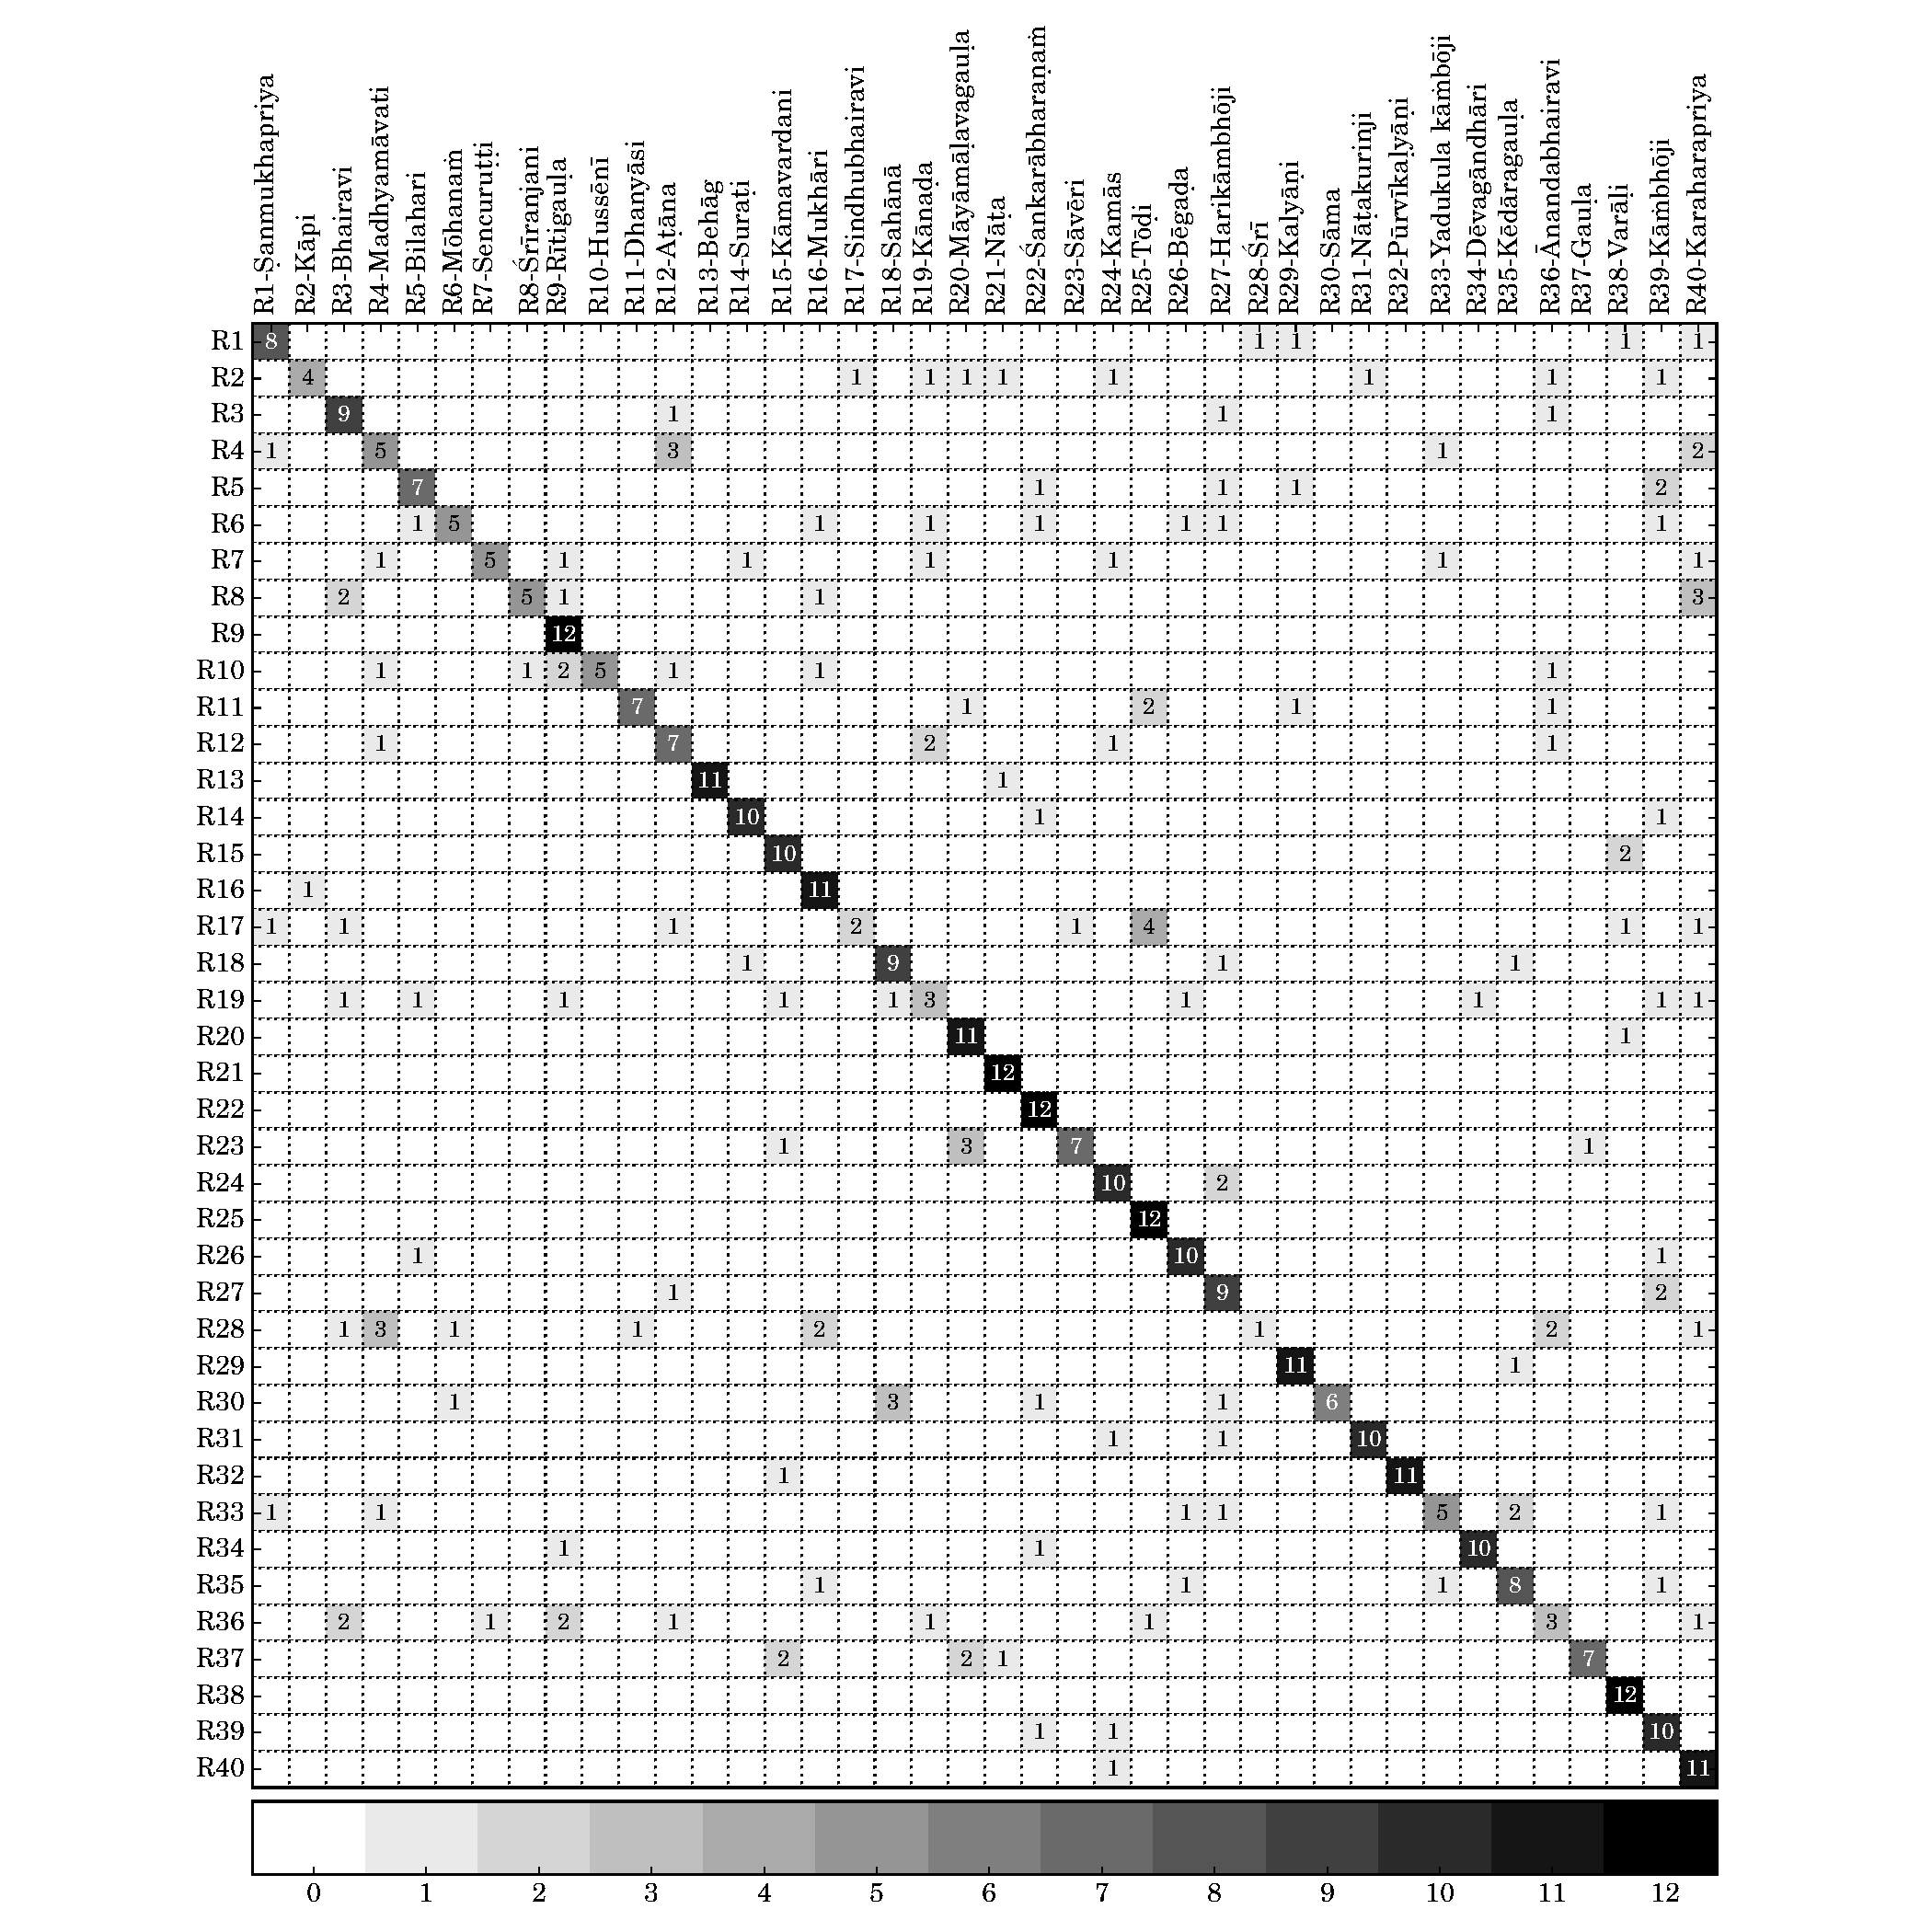
\includegraphics[width=\figSizeNinety]{ch07_ragaRecognition/figures/CM_vsm_cmd_var1.pdf}
	\end{center}
	\caption{Confusion matrix of the \gls{raga} predictions by \acrshort{sotaChordia} on \acrshort{rrds_cmd_big} dataset. The different shades of grey are mapped to different number of audio recordings.}
	\label{fig:confusion_matrix_cmd_chordia}
\end{figure}

\begin{figure}[h]
	\begin{center}
		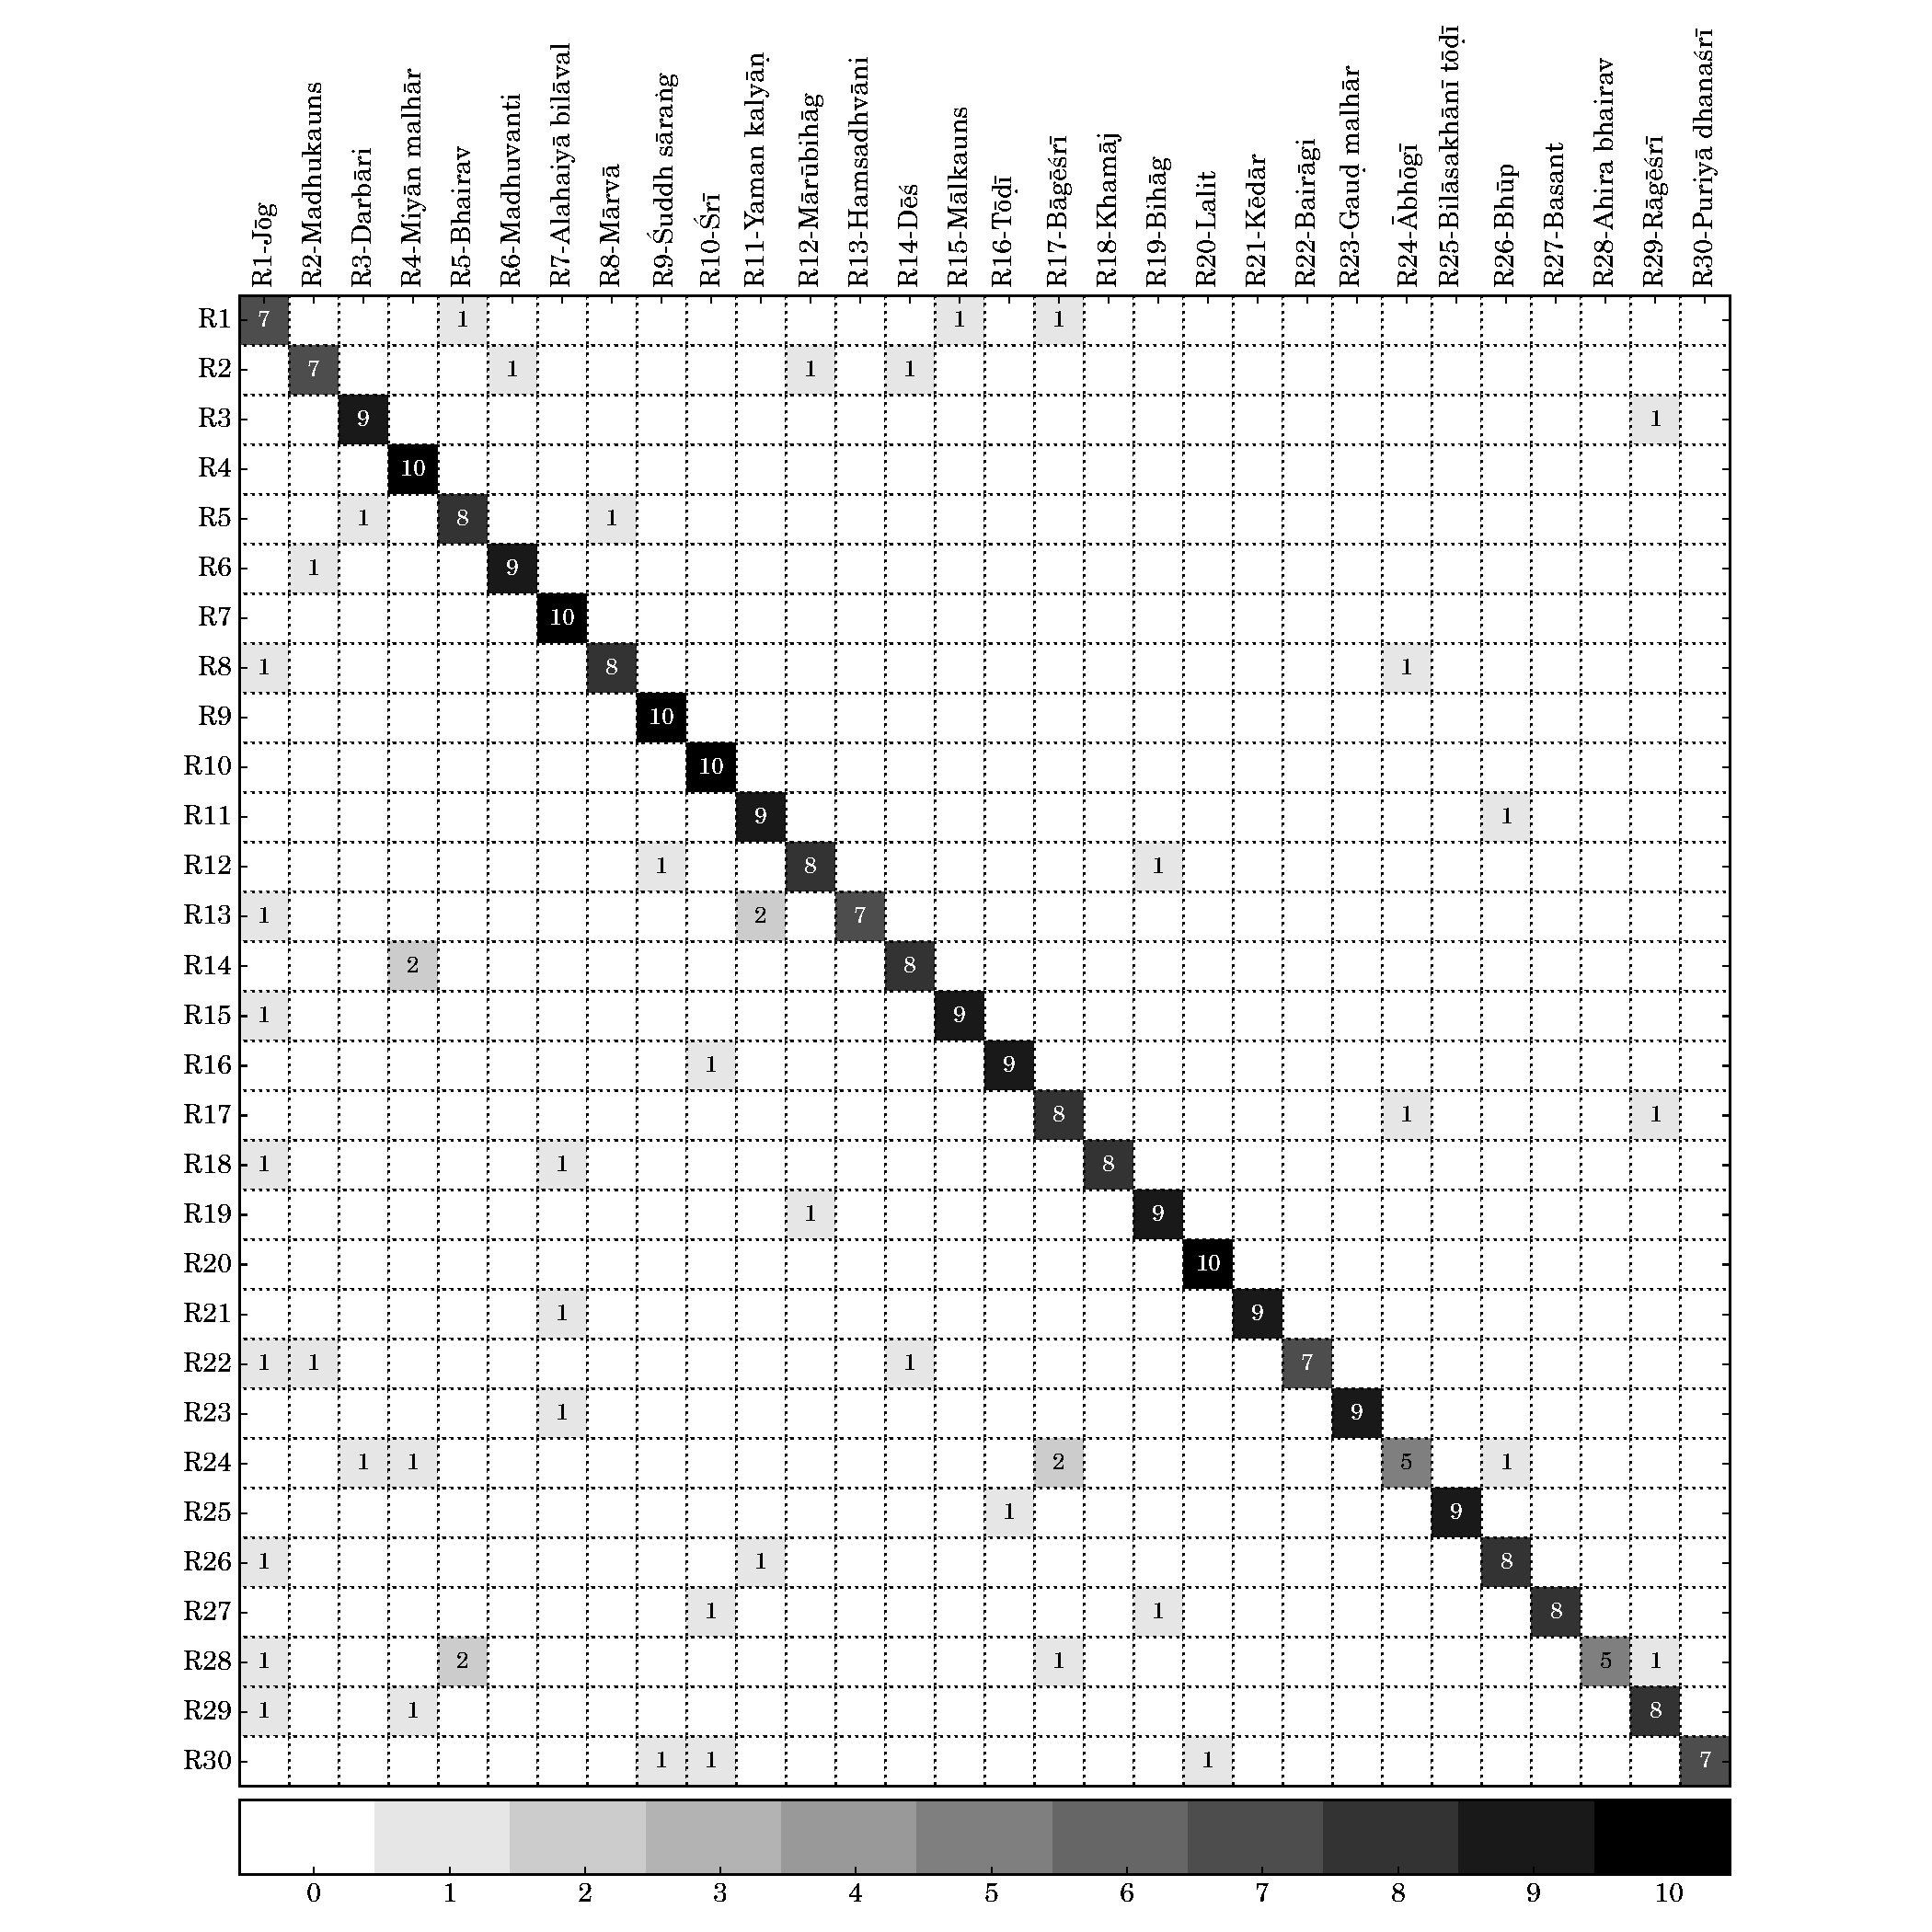
\includegraphics[width=\figSizeNinety]{ch07_ragaRecognition/figures/CM_vsm_hmd_var1.pdf}
	\end{center}
	\caption{Confusion matrix of the \gls{raga} predictions by \acrshort{sotaChordia} on \acrshort{rrds_hmd_big} dataset. The different shades of grey are mapped to different number of audio recordings.}
	\label{fig:confusion_matrix_hmd_chordia}
\end{figure}



\begin{figure}[h]
	\begin{center}
		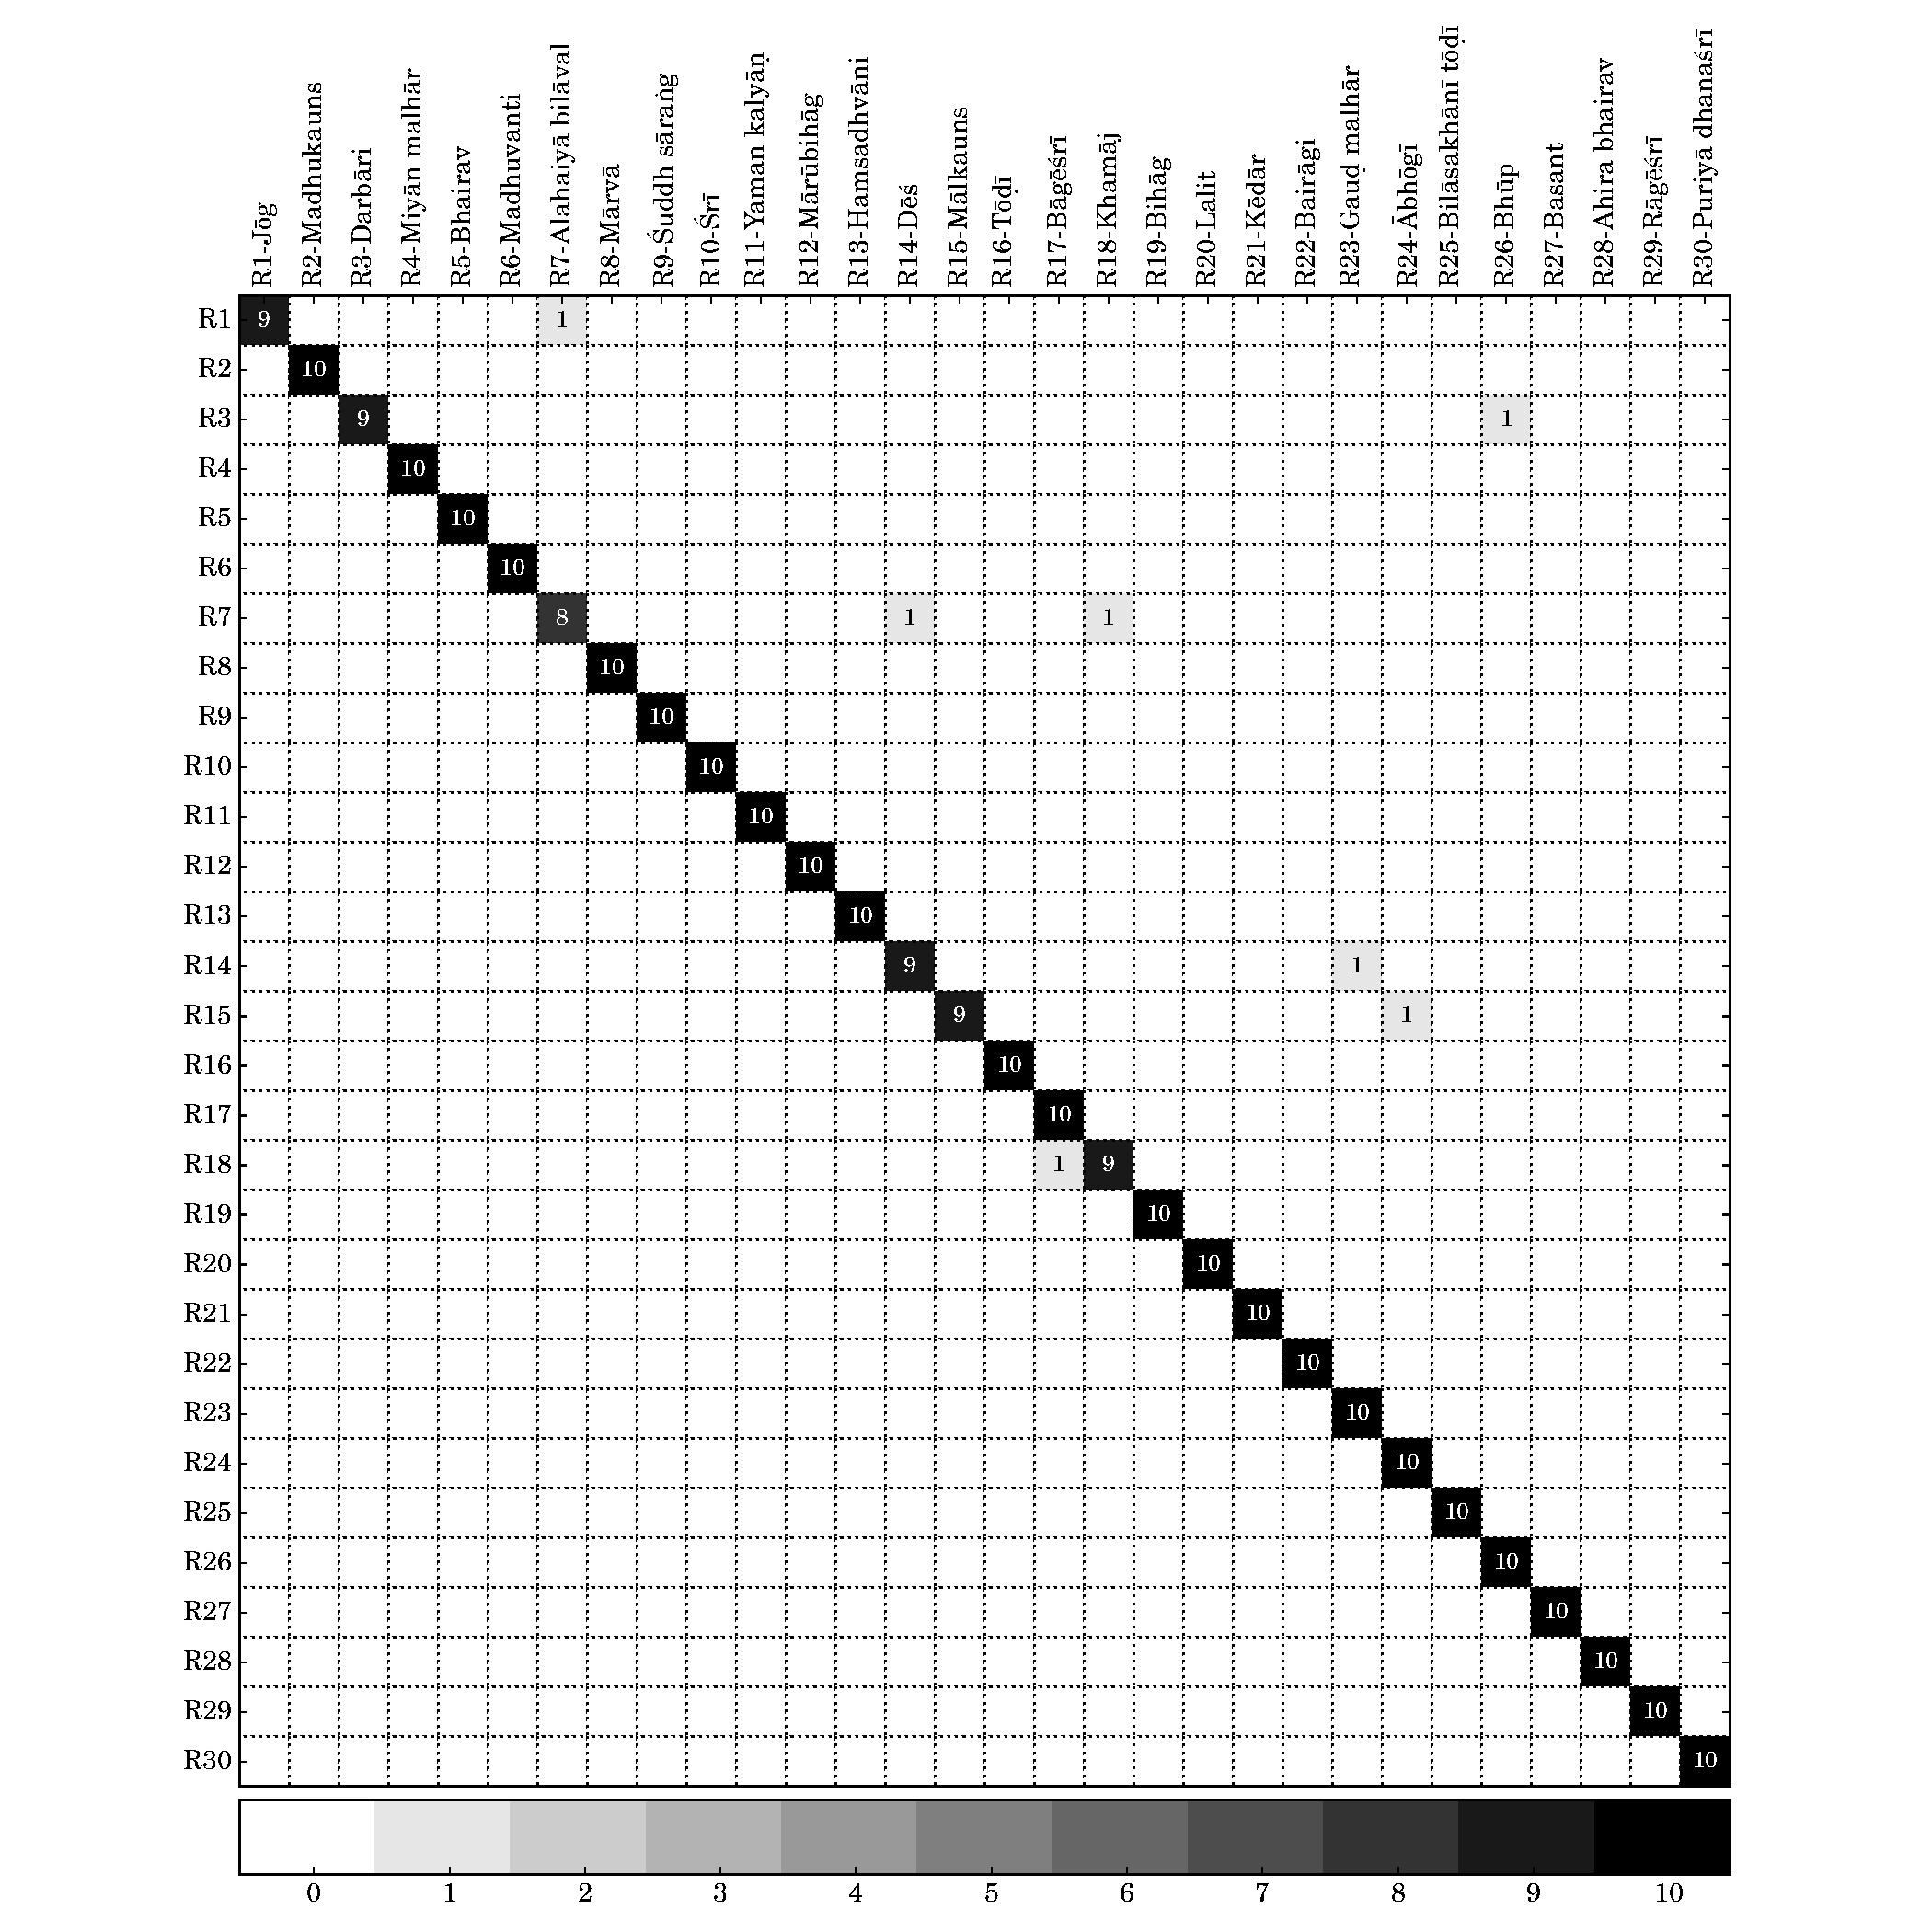
\includegraphics[width=\figSizeNinety]{ch07_ragaRecognition/figures/CM_tdms_hmd_var1.pdf}
	\end{center}
	\caption{Confusion matrix of the \gls{raga} predictions by \acrshort{ragarecTDMS} on \acrshort{rrds_hmd_big} dataset. The different shades of grey are mapped to different number of audio recordings.}
	\label{fig:confusion_matrix_hmd_tdms}
\end{figure}


